% This text is proprietary.
% It's a part of presentation made by myself.
% It may not used commercial.
% The noncommercial use such as private and study is free
% Dec 2007
% Author: Sascha Frank 
% University Freiburg 
% www.informatik.uni-freiburg.de/~frank/
%
% 
\documentclass{beamer}
\setbeamertemplate{navigation symbols}{}

%\setbeamercolor{frametitle}{fg=black,bg=white}
%\setbeamercolor{title}{fg=black,bg=yellow!85!orange}
\usetheme{AnnArbor}
\usecolortheme{beaver}
\usefonttheme{structurebold}

\beamersetuncovermixins{\opaqueness<1>{25}}{\opaqueness<2->{15}}
\begin{document}
\title{Community Detection}
\subtitle{In Large Networks}
\author{June Andrews}
\date{\today} 

\begin{frame}
\titlepage
\end{frame}


\begin{frame}\frametitle{Thanks!}
It goes without saying, these people have been inspiring forces of nature to work with:
\begin{itemize}
\item Mr. Len Kulbacki
\item Coach Wilson
\item Dr. James Sethian
\item Patricia Kovatch
\item Dr. Alex Vladimirsky
\item Dr. John Hopcroft
\item Dr. Steve Strogatz (thanks to Prof Rand for acting proxy :)
\item Dr. Jon Kleinberg
\end{itemize}

\begin{figure}

\includegraphics[width=.7in]{Figures/nsflogo} 
\caption{Thanks to the NSF Graduate Fellowship Program!}
\end{figure}

\end{frame}

\begin{frame}\frametitle{Table of contents}\tableofcontents
\end{frame} 


\section{Motivation}

\begin{frame}\frametitle{Dolphins}
Dolphins form pods.
\begin{figure}
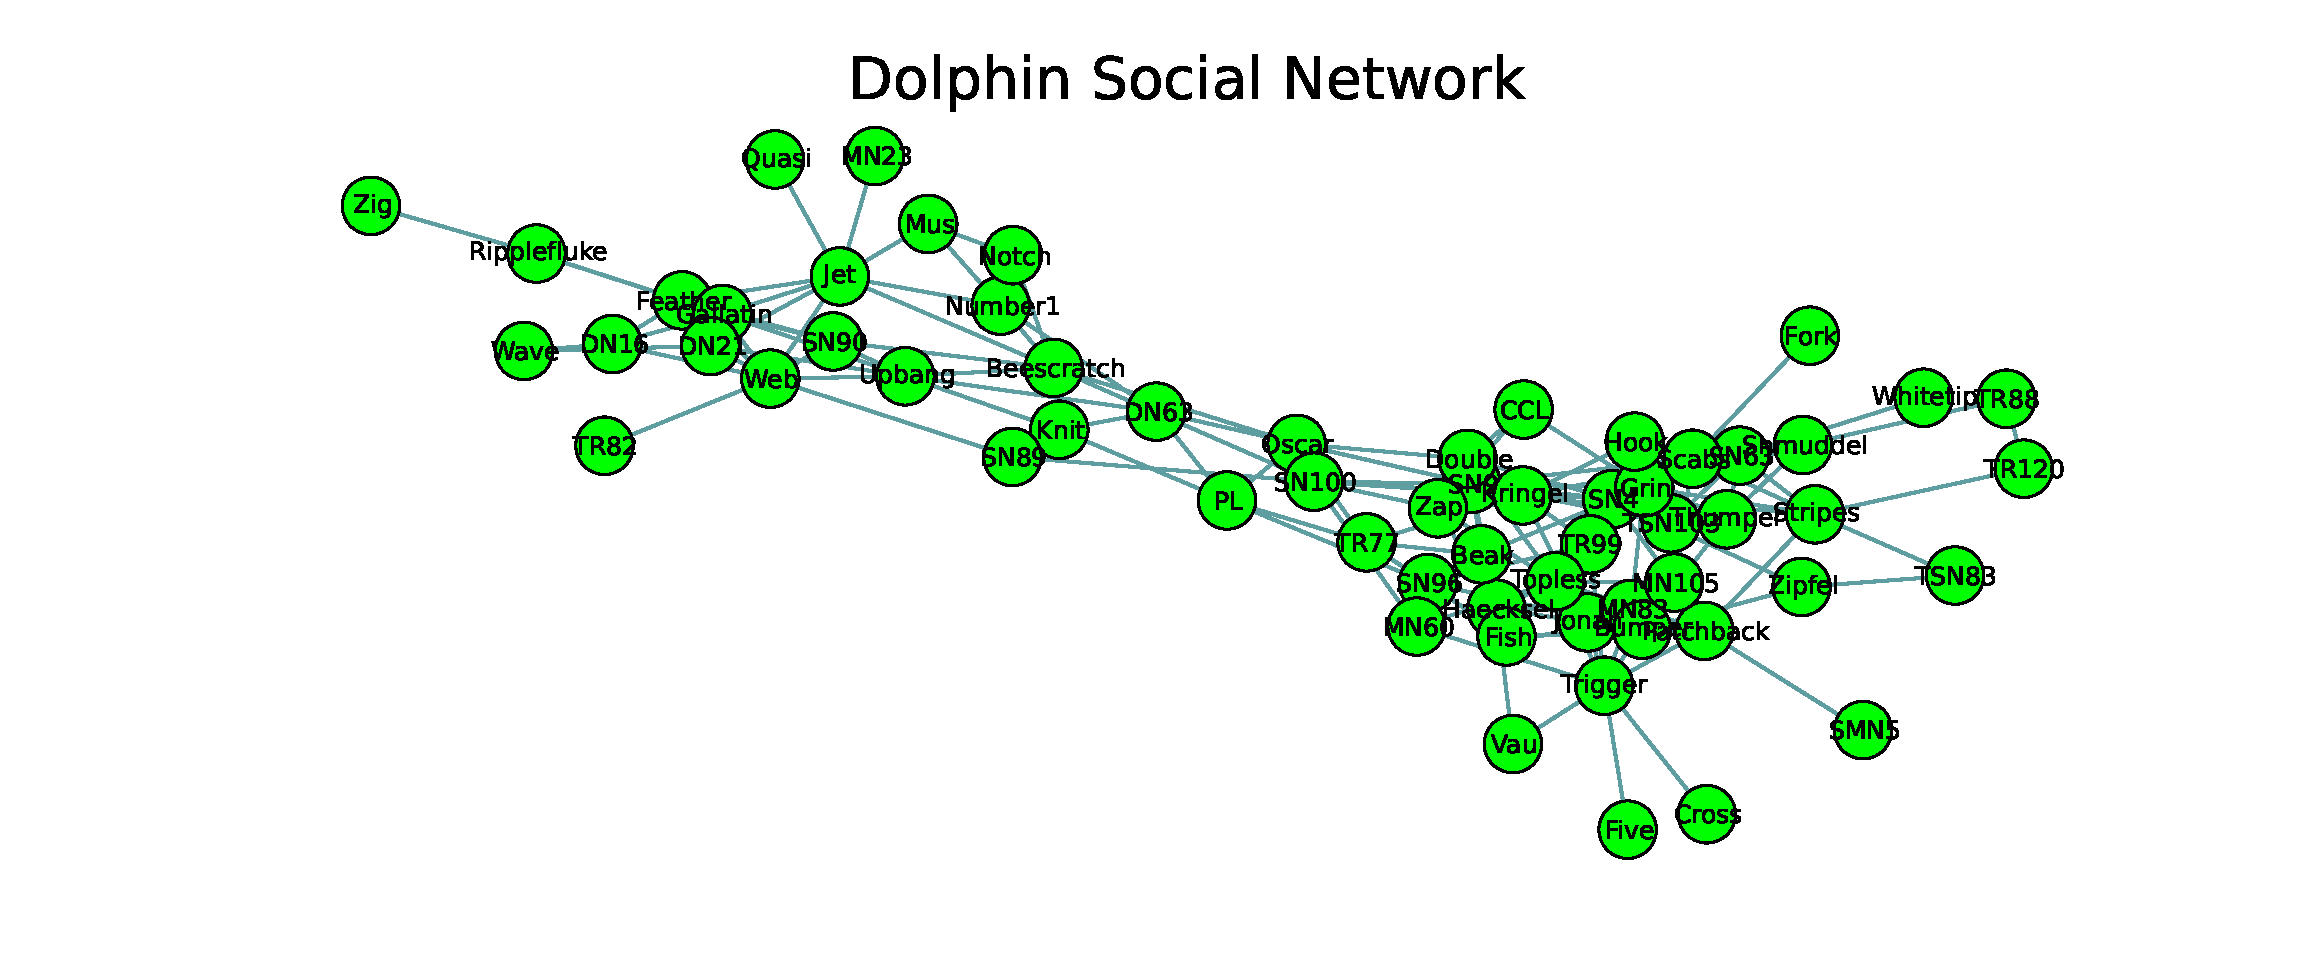
\includegraphics[width=5in]{Figures/dolphin_social_network}
\caption{Nodes are dolphins.  Edges are dolphins seen together.}
\end{figure}
\end{frame}

\begin{frame}\frametitle{Dolphins}
If we know what the pods are:
\begin{itemize}
\item Who are the dolphins that interact between pods?
\item How often do pods interact?
\item Do the pods have a dominant leader?
\end{itemize}
\begin{figure}
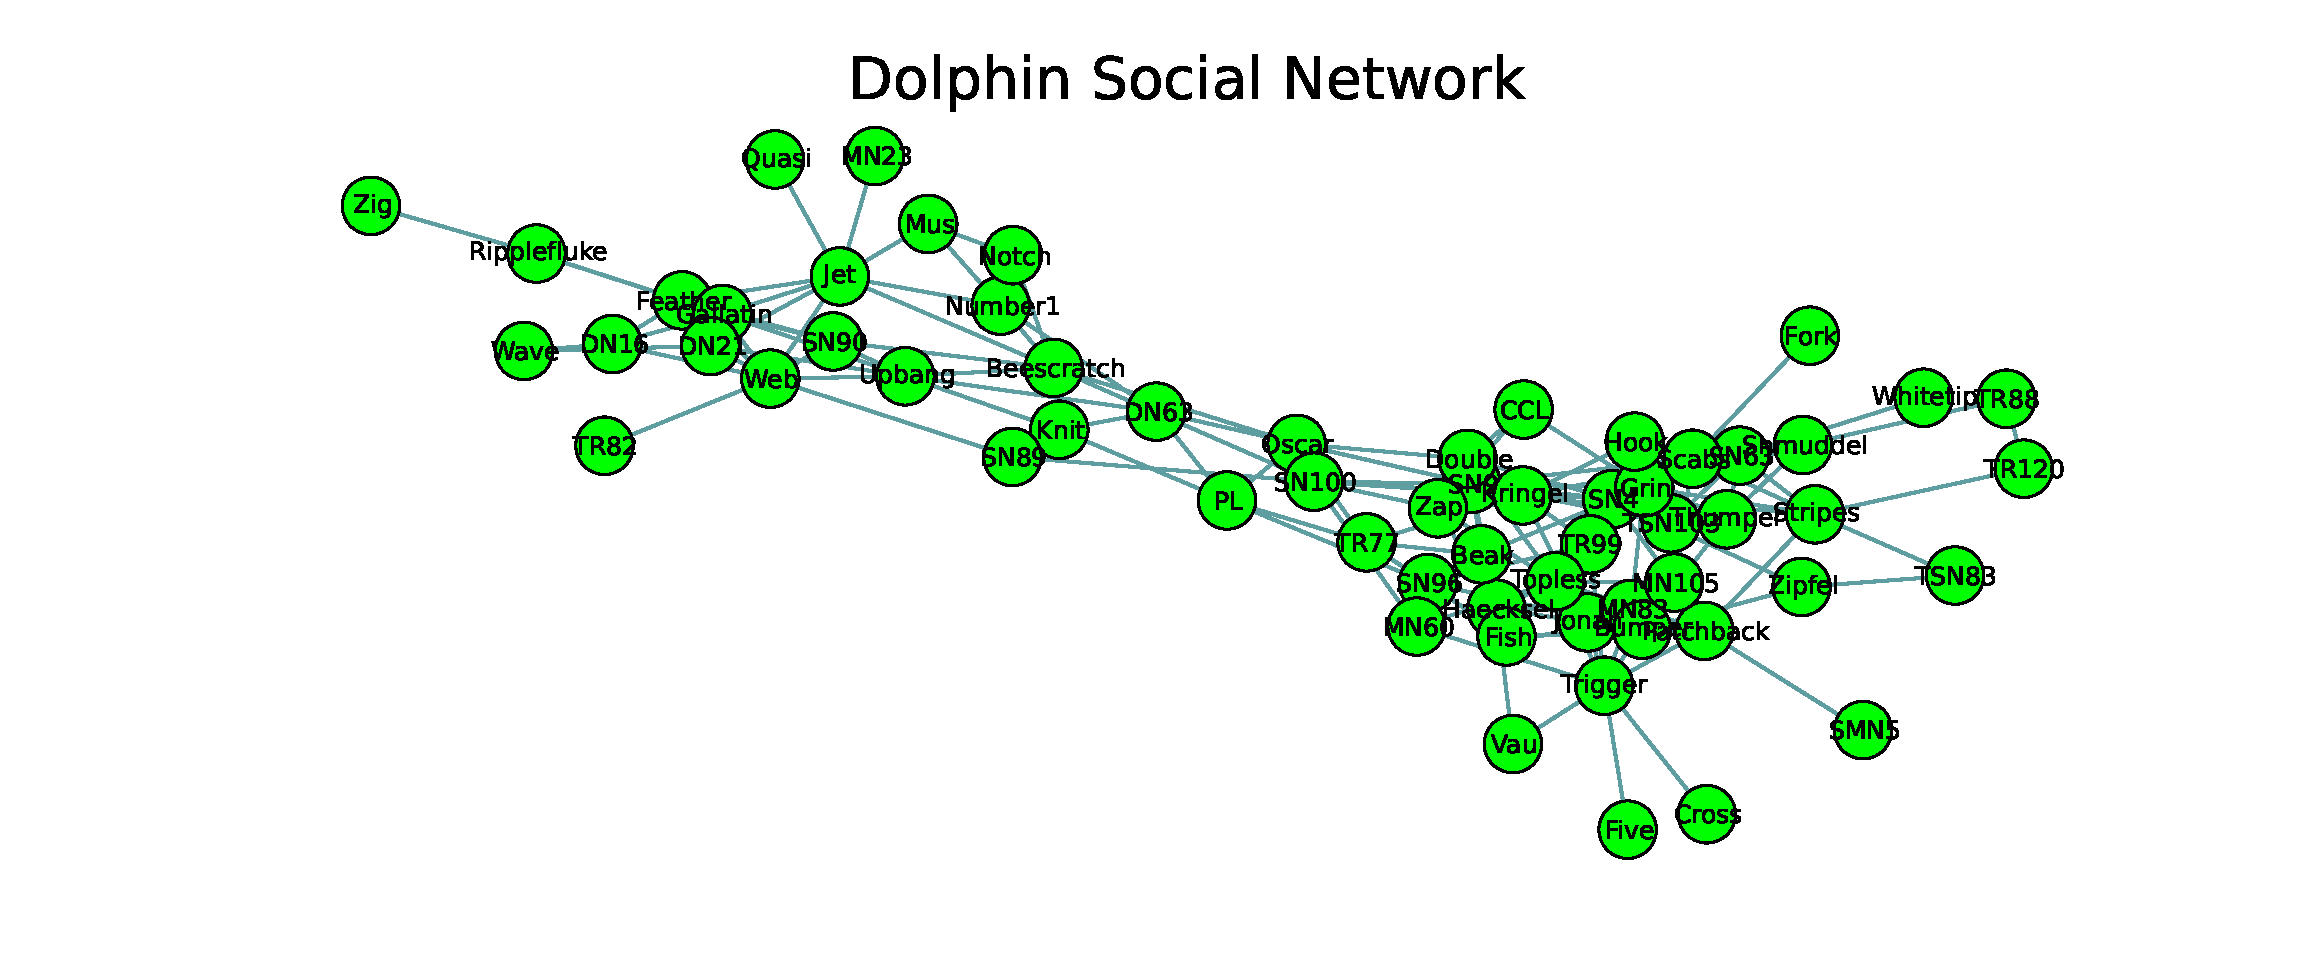
\includegraphics[width=3in]{Figures/dolphin_social_network}
\end{figure}
\end{frame}


\begin{frame}\frametitle{Karate Club}
People are members of a group.
\begin{figure}
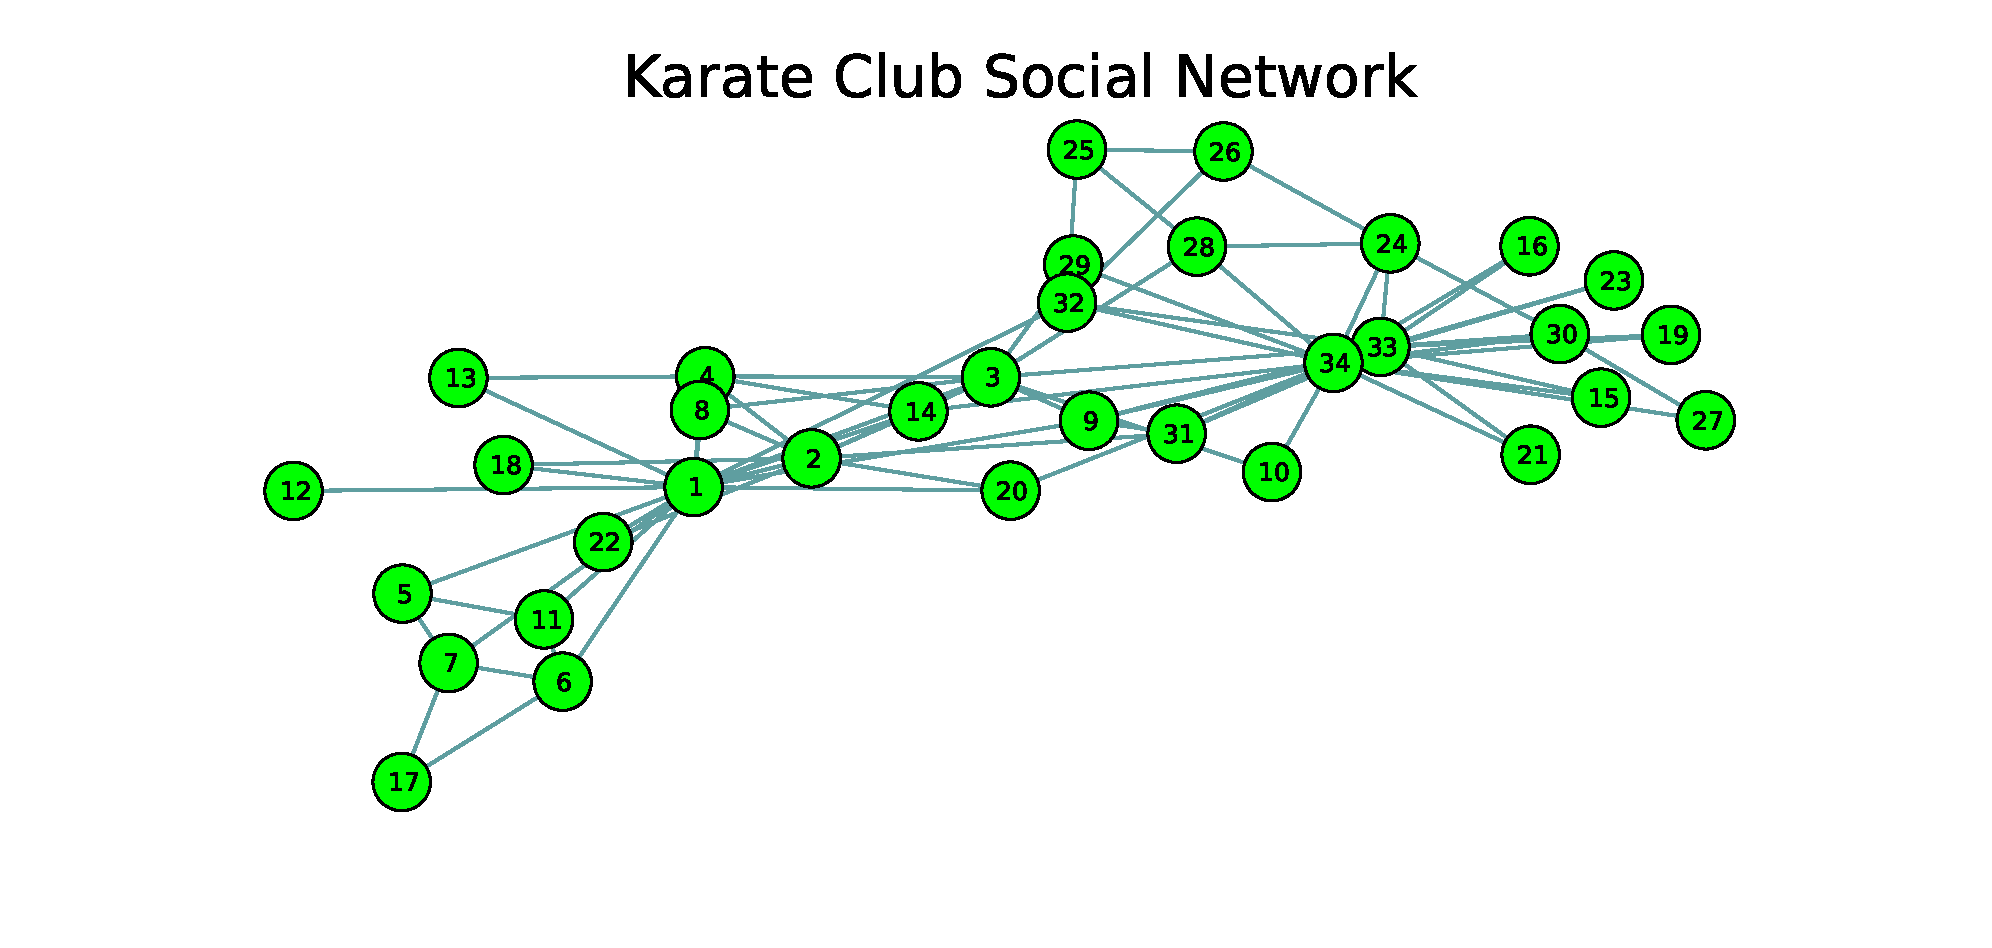
\includegraphics[width=4.5in]{Figures/karate_social_network}
\caption{Nodes are students.  Edges are students seen outside of class together.}
\end{figure}
\end{frame}



\begin{frame}\frametitle{Karate Club}
If we know the groups people form:
\begin{itemize}
\item If something happens to split the social network, which people will do what?
\item How many groups is someone a member of?
\item Who are the influential members of a group?
\end{itemize}
\begin{figure}
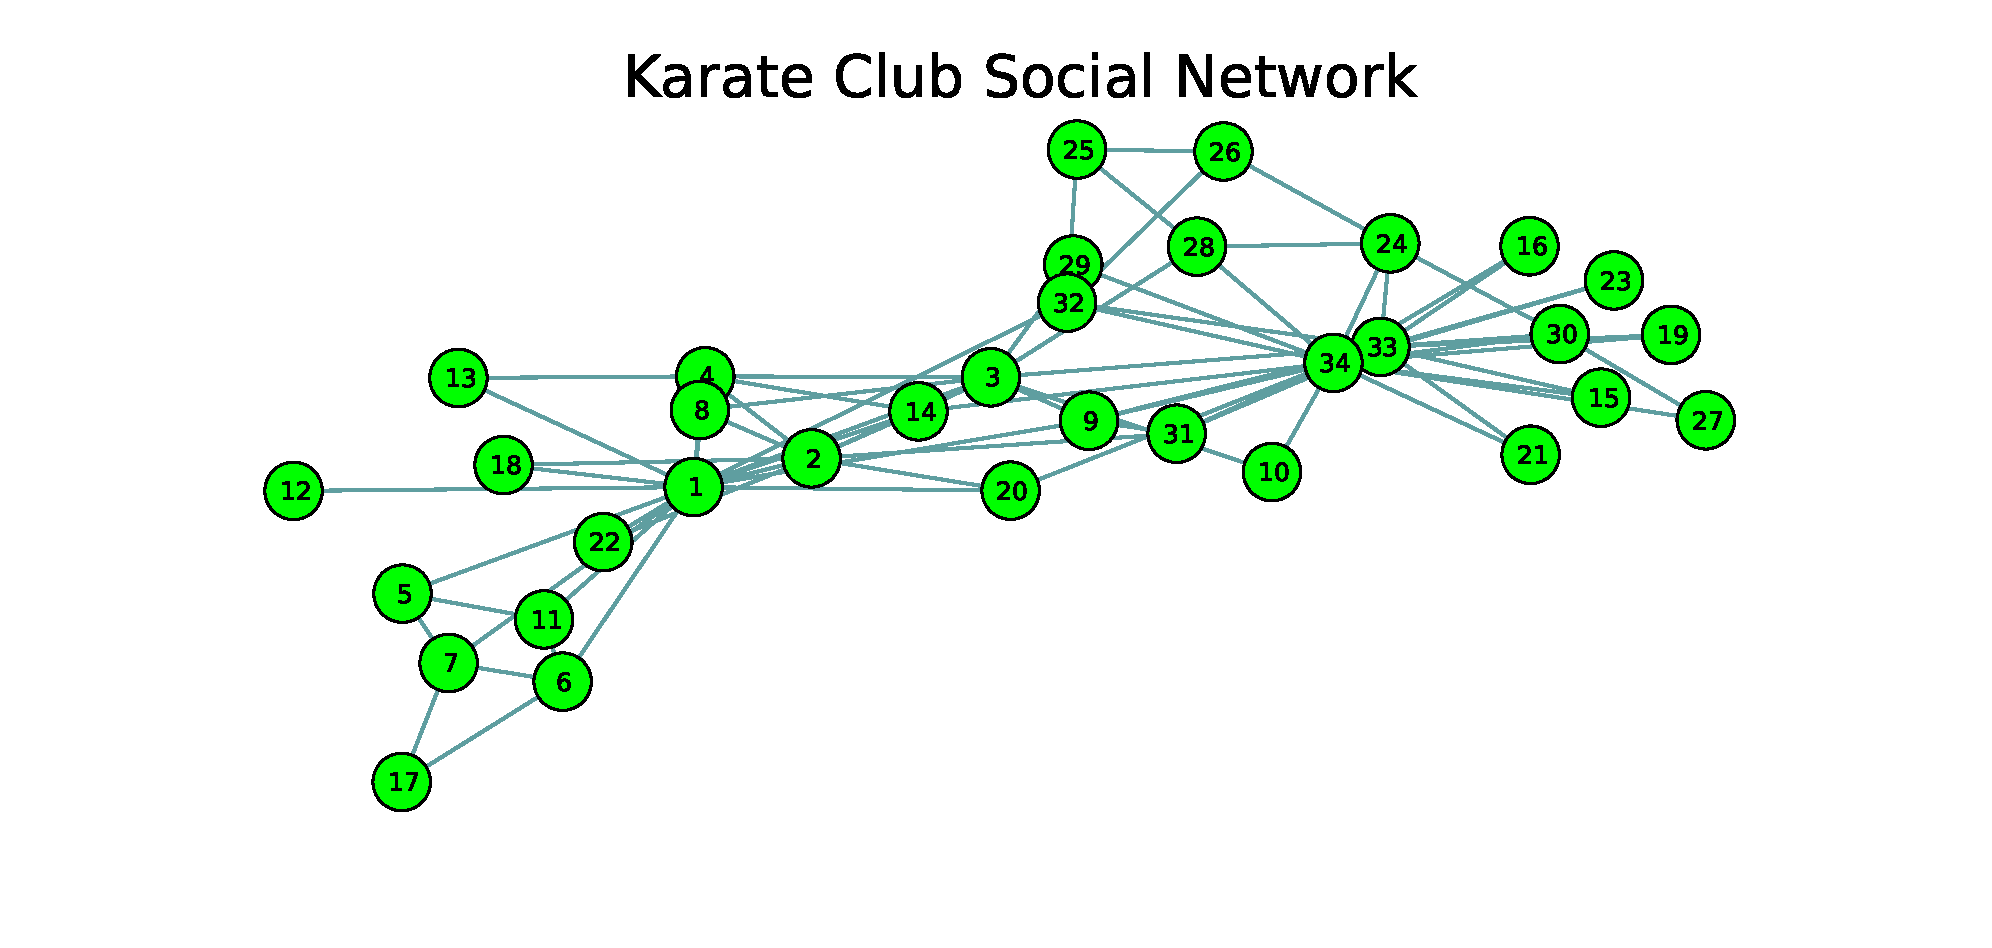
\includegraphics[width=3in]{Figures/karate_social_network}
\end{figure}
\end{frame}


\begin{frame}\frametitle{In General}

JTODO insert figure of:
Build Network $\rightarrow$ Find Communities $\rightarrow$ Analyze

\begin{block}{}
\begin{center}
How do you detect communities?
\end{center}
\end{block}

\end{frame}

\begin{frame}\frametitle{Science on Networks}

Many applications have developed their own methods.

\begin{table}[!h]
\centering
\begin{tabular}{l|l}
Application & Community Detection Method \\ \hline
Computation Distribution & Recursive Bi-section [Karypis \& Kumar] \\
Statistical Mechanics & Belief Propogation [Hastings]\\
Storage of Large Matrices & Local Spectral Analysis [Andersen \& Chung] \\
Taxonomy & Neighbor Joining [Saitou \& Nei] \\
$\vdots$ & $\vdots$
\end{tabular}
\end{table}

\begin{block}{}
\begin{center}
How do we compare them?
\end{center}
\end{block}

\end{frame}

\begin{frame}\frametitle{This Talk}
\begin{center}
\begin{itemize}
\item Create a way to understand Community Detection Methods.
\item Create a method to handle large complex networks.
\item Demonstrate power of new method on:
	\begin{enumerate}
		\item Wikipedia Elections 
		\item Physics Archive Citation Network
	\end{enumerate}
\end{itemize}
\end{center}

\end{frame}


\section{Past Work}


\begin{frame}\frametitle{Brief Terminology}

\begin{definition}[Internal Edges]
Edges between members of the same community.
\end{definition}
JTODO include diagram of edges
\begin{definition}[External Edges]
Edges between members of different communities.
\end{definition}
\end{frame}


\begin{frame}\frametitle{Previous Community Detection Methods}

Pick a definition of a Community and then find it.
\begin{itemize}
\item $(\alpha, \beta)$ communities, every node in $C$ is connected by at least $\beta$ internal edges, every node outside of $C$ is connected by at most $\alpha$ edges. [Mishra et al]
\item Modularity, more internal edges than expected in a random graph. [Newman]
\item Conductance, a step in a random walk will probabilistically stay within the community. [JTODO]
\item Edge Betweenness, remove external edges to reveal communities. [Girvan \& Newman]
\item $\cdots$
\end{itemize}

\end{frame}


\section{Metrics for a Single Community}


\begin{frame}\frametitle{Dection For Single Communities}
Let's not define a community just yet.
\newline
\newline
Our approach:
\begin{itemize}
\item What are the desired characteristics of a community?
\item Find a community with the best characteristics.
\end{itemize}

\end{frame}



\begin{frame}\frametitle{Characteristics of Single Communities}
\begin{itemize}
\item {\sc Internal Density} is density of edges within the community.
\item {\sc External Density} is the density of edges leaving the community.
\item {\sc Size} of the community.
\item {\sc Diameter} of the community.
\item {\sc Average Shortest Path} within the community.
\item {\sc Out Degree Fraction}, {\sc Degree Distribution},  $\cdots$
\end{itemize}

\begin{block}{Representative Characteristics}
\begin{center}
All of the listed characteristics can be bounded by {\sc Internal Density}, {\sc External Density}, and {\sc Size}.
\end{center}
\end{block}
\end{frame}



\begin{frame}\frametitle{The 3D space of Communities}
Given a metric $M$ that evaluates communities in the $(I(C), E(C), |C|)$ space, let us find

If networks were in a continuous space, we could use gradients to maximize metric.

\end{frame}



\begin{frame}\frametitle{Conductance}

Level sets of Conductance.

\end{frame}


\begin{frame}\frametitle{New Metric for a Single Community}

Level sets of 

\end{frame}




\begin{frame}\frametitle{Algorithmcs in the IE space}

Running algorithms in the IE space.

\end{frame}



\section{Metrics for a Set of Communities}

\begin{frame}\frametitle{Characteristics of Sets of Communities}

Many characteristics, again defined by internal density, external density, and size of set.

\end{frame}


\begin{frame}\frametitle{The 3D space of Communities}

Consider level sets of how a metric divides the space.

If continuous use gradient to maximize metric.

\end{frame}



\begin{frame}\frametitle{Modularity}

Level sets of Modularity.

\end{frame}



\begin{frame}\frametitle{New Metric for a Single Community}

Level sets of 

\end{frame}

\begin{frame} \frametitle{Algorithm for maximizing new metric}

Conjecture, once you decrease int density, never go back

set $a=1$ and increment $b$, and $c$.

Use the Louvain algorithm for maximizing the metric at each stage.

\end{frame}

\begin{frame}\frametitle{Algorithmcs in the IES space}

Running algorithms in the IES space.

\end{frame}


\section{Parallel Technique}



\begin{frame}\frametitle{Future}

Networks are getting big.

Before we asked the question of, is this a good set of communities.

Now we need to ask does this node and set of nodes belong to a community?

Why?  No communication in parallelization.

\end{frame}

\begin{frame}\frametitle{Characteristics}

The two characteristics between a node and a set of nodes are $\chi_e$ and $\chi_p$.

\end{frame}

\begin{frame}\frametitle{Community}

How do we know we have a community?

Closure.

\end{frame}


\begin{frame}\frametitle{Algorithm}

\begin{itemize}
\item Find the seeds
\item Expand the seeds
\end{itemize}


\end{frame}


\begin{frame}\frametitle{Seeds}

Pick a set of nodes we know must belong to the same community.

Find very dense sets of nodes, presume begin with a clique, and expand into the local neighborhood.

If seeds are distance 2 apart will be in the same community, if the community is large.

\end{frame}



\begin{frame}\frametitle{Expansion}

\end{frame}


\begin{frame}\frametitle{Correctness of Expansion}

Probability of Correctness.

\end{frame}



\begin{frame}\frametitle{Algorithms}

\end{frame}


\section{Applications}


\begin{frame}\frametitle{Checkpoint}

We have new methods. 

We'll leave comparisons to known methods to the thesis.

We'll do a sanity check against known communities and then present results from applications that could not have been done before.
\end{frame}


\subsection{Known Communities}

\begin{frame}\frametitle{Test on Dolphins}

\end{frame}


\begin{frame}\frametitle{Test on Karate}

\end{frame}


\subsection{Physics Archive}



\begin{frame}\frametitle{Physics Archive}
The more communities a paper is immediately popular in the more citations that paper will get.

Correlated with cross community journals - confirm.
\end{frame}


\subsection{Wikipedia Voting}

\begin{frame}\frametitle{Wikipedia Voting}

JTODO include picture of what it is

\end{frame}


\begin{frame}\frametitle{Communities Predicting a User's Vote}
Communities are sets of user with similar voting patterns.  There are $\approx 600$ communities covering $JTODO \%$ of the nodes.
\newline
\newline

\begin{block}{Vote Prediction}
\begin{center}
Given the communities a user is in, we can predict a user's vote with $86\%$ accuracy.
\end{center}
\end{block}
 This is close to Kleinberg et al's work of $90 \%$ accuracy.

\end{frame}

\begin{frame}\frametitle{Communities Predicting an Election's Outcome.}
Users campaign to sets of communities, but not everyone from a community votes.  If they did:

\begin{block}{Election Prediction}
\begin{center}
Given the Communities in Wiki Voting Similiarities, $14\%$ of election results would be over turned.
\end{center}
\end{block}

\end{frame}


\end{document}










% sample code to work with



\section{Section no.1} 
\begin{frame}\frametitle{Title} 
Each frame should have a title.
\end{frame}
\subsection{Subsection no.1.1  }
\begin{frame} 
Without title somethink is missing. 
\end{frame}


\section{Section no. 2} 
\subsection{Lists I}
\begin{frame}\frametitle{unnumbered lists}
\begin{itemize}
\item Introduction to  \LaTeX  
\item Course 2 
\item Termpapers and presentations with \LaTeX 
\item Beamer class
\end{itemize} 
\end{frame}

\begin{frame}\frametitle{lists with pause}
\begin{itemize}
\item Introduction to  \LaTeX \pause 
\item Course 2 \pause 
\item Termpapers and presentations with \LaTeX \pause 
\item Beamer class
\end{itemize} 
\end{frame}

\subsection{Lists II}
\begin{frame}\frametitle{numbered lists}
\begin{enumerate}
\item Introduction to  \LaTeX  
\item Course 2 
\item Termpapers and presentations with \LaTeX 
\item Beamer class
\end{enumerate}
\end{frame}

\begin{frame}\frametitle{numbered lists with pause}
\begin{enumerate}
\item Introduction to  \LaTeX \pause 
\item Course 2 \pause 
\item Termpapers and presentations with \LaTeX \pause 
\item Beamer class
\end{enumerate}
\end{frame}

\section{Section no.3} 
\subsection{Tables}
\begin{frame}\frametitle{Tables}
\begin{tabular}{|c|c|c|}
\hline
\textbf{Date} & \textbf{Instructor} & \textbf{Title} \\
\hline
WS 04/05 & Sascha Frank & First steps with  \LaTeX  \\
\hline
SS 05 & Sascha Frank & \LaTeX \ Course serial \\
\hline
\end{tabular}
\end{frame}


\begin{frame}\frametitle{Tables with pause}
\begin{tabular}{c c c}
A & B & C \\ 
\pause 
1 & 2 & 3 \\  
\pause 
A & B & C \\ 
\end{tabular} 
\end{frame}


\section{Section no. 4}
\subsection{blocs}
\begin{frame}\frametitle{blocs}

\begin{block}{title of the bloc}
bloc text
\end{block}

\begin{exampleblock}{title of the bloc}
bloc text
\end{exampleblock}


\begin{alertblock}{title of the bloc}
bloc text
\end{alertblock}
\end{frame}

\section{Section no. 5}
\subsection{split screen}

\begin{frame}\frametitle{splitting screen}
\begin{columns}
\begin{column}{5cm}
\begin{itemize}
\item Beamer 
\item Beamer Class 
\item Beamer Class Latex 
\end{itemize}
\end{column}
\begin{column}{5cm}
\begin{tabular}{|c|c|}
\hline
\textbf{Instructor} & \textbf{Title} \\
\hline
Sascha Frank &  \LaTeX \ Course 1 \\
\hline
Sascha Frank &  Course serial  \\
\hline
\end{tabular}
\end{column}
\end{columns}
\end{frame}

\subsection{Pictures} 
\begin{frame}\frametitle{pictures in latex beamer class}
\begin{figure}
\includegraphics[scale=0.5]{PIC1} 
\caption{show an example picture}
\end{figure}
\end{frame}

\subsection{joining picture and lists} 

\begin{frame}
\frametitle{pictures and lists in beamer class}
\begin{columns}
\begin{column}{5cm}
\begin{itemize}
\item<1-> subject 1
\item<3-> subject 2
\item<5-> subject 3
\end{itemize}
\vspace{3cm} 
\end{column}
\begin{column}{5cm}
\begin{overprint}
\includegraphics<2>{PIC1}
\includegraphics<4>{PIC2}
\includegraphics<6>{PIC3}
\end{overprint}
\end{column}
\end{columns}
\end{frame}


\subsection{pictures which need more space} 
\begin{frame}[plain]
\frametitle{plain, or a way to get more space}
\begin{figure}
\includegraphics[scale=0.5]{PIC1} 
\caption{show an example picture}
\end{figure}
\end{frame}
